\section{Overview of Supervised Learning}

%2.1
\begin{sol}
Since
\[
\hat{k}\triangleq\argmin_k\|t_k-\hat{y}\|=\argmin_k\|t_k-\hat{y}\|^2=\argmin_k\sum_{i\ne k}\hat{y}_i^2+(1-\hat{y}_k)^2
\]
and elements of $\hat{y}$ sum to one, so if $\hat{y}_k$ goes larger, both $\sum_{i\ne k}\hat{y}_i^2$ and $(1-\hat{y}_k)^2$ will get smaller, which means $\hat{k}=\argmax_k\hat{y}_i$ 
\end{sol}

%2.2
\begin{sol}
The boundary satisfies $\{x\mid \Pr(C=\mathrm{Orange}\vert X=x) =\Pr(C=\mathrm{Blue}\vert X=x)\}$. Suppose $\{m_k^C\}_{k=1}^{10}$ are known. Now introduce a latent variable $h$ for the index of the selected $m^C$. We have
\begin{align*}
\Pr(C\vert X) =& \frac{\Pr(X\vert C)\Pr(C)}{\sum_C\Pr(X\vert C)\Pr(C)}\\
\Pr(X\vert C) =& \Pr(X\vert C,\{m_i^C\})\\
=& \sum_h\Pr(X\vert C,h,m_h^C)\Pr(h\vert C,\{m_i^C\})\\
=& \sum_h\Pr(X\vert m_h^C)\Pr(h)\\
\Pr(X\vert m_h^C) =& \mathcal{N}(m_h^C,\mathbf{I}/5)\\
\Pr(h) =& \frac{1}{10}\\
\Pr(C) =& \frac{1}{2}
\end{align*}
So the boundary can be further simplified as
\[
\left\{x\biggm| \sum_{k=1}^{10} \mathcal{N}(m_k^\mathrm{Orange},\mathbf{I}/5)=\sum_{k=1}^{10} \mathcal{N}(m_k^\mathrm{Blue},\mathbf{I}/5)\right\}
\]

Figure \ref{fig:2-2} gives an example.

\begin{figure}
	\centering
	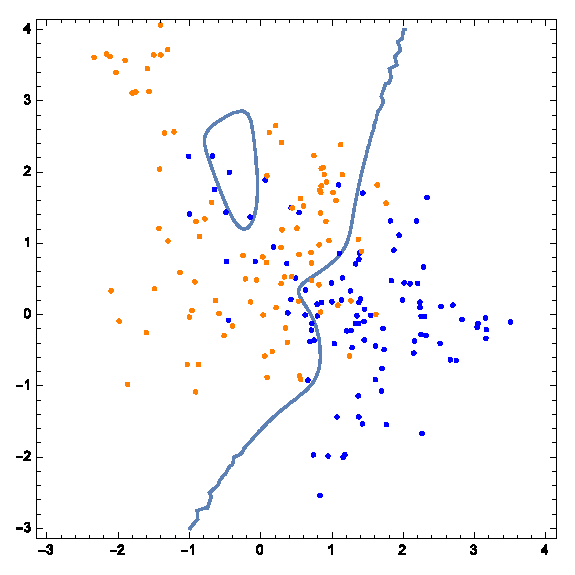
\includegraphics[width=\textwidth]{figures/2_2.eps}
	\caption{An example of the boundary.}
	\label{fig:2-2}
\end{figure}

\end{sol}

%2.3
\begin{sol}
By spherical coordinates, the volume element is \[
dV=r^{p-1}\sin^{p-2}\phi_1\cdots\sin\phi_{p-2}\,drd\phi_1\cdots d\phi_{p-2}d\phi_{p-1}
\]
So $r$'s probability density function $f(r)\propto r^{p-1}$. Further we have $f(r)=pr^{p-1}$ and the cumulative distribution function $F(r)=r^p$. According to order statistic, the distribution of the minimum among $N$ samples is
\begin{align*}
f_{(1)}(r) =& N\left[1-F(r)\right]^{N-1}f(r)\\
=& pN\left(1-r^p\right)^{N-1}r^{p-1}
\end{align*}
The median $r_0$ then satisfies
\begin{align*}
& \int_0^{r_0}f_{(1)}(r)\,dr=\int_{r_0}^1f_{(1)}(r)\,dr \\
\Longrightarrow & \int_0^{r_0^p}\left(1-r^p\right)^{N-1}\,dr^p=\int_{r_0^p}^1\left(1-r^p\right)^{N-1}\,dr^p \\
\Longrightarrow & 1-\left(1-r_0^p\right)^N=\left(1-r_0^p\right)^N \\
\Longrightarrow & r_0=\left[1-\left(\frac{1}{2}\right)^{\frac{1}{N}}\right]^{\frac{1}{p}}
\end{align*}
\end{sol}

%2.4
\begin{sol}
\begin{align*}
x\sim\mathcal{N}(0,\mathbf{I}_p)\Longrightarrow & z=\Tr{a}x\sim\mathcal{N}(\Tr{a}0,\Tr{a}\mathbf{I}_pa)=\mathcal{N}(0,1)\\
\Longrightarrow & z^2\sim \chi_1^2
\end{align*}
\end{sol}

%2.5
\begin{sol}
Given an arbitrary test point $x_0$, the corresponding ground truth $y_0=\Tr{x_0}\beta+\epsilon_0$ and the estimation $\hat{y}_0=\Tr{x_0}\hat{\beta}$, we have
\begin{align*}
\mathrm{EPE}(x_0) = & \E_{y_0\vert x_0}\E_{\mathcal{T}}(y_0-\hat{y}_0)^2\\
=& \E_{y_0\vert x_0}\E_{\mathcal{T}}\left[(y_0-\Tr{x_0}\beta)-(\hat{y}_0-\E_\mathcal{T}\hat{y}_0)-(\E_\mathcal{T}\hat{y}_0-\Tr{x_0}\beta)\right]^2 \\
=& \E_{y_0\vert x_0}(y_0-\Tr{x_0}\beta)^2+\E_{\mathcal{T}}(\hat{y}_0-\E_\mathcal{T}\hat{y}_0)^2+(\E_\mathcal{T}\hat{y}_0-\Tr{x_0}\beta)^2 \\
& -2 \E_{y_0\vert x_0}(y_0-\Tr{x_0}\beta) \E_{\mathcal{T}}(\hat{y}_0-\E_\mathcal{T}\hat{y}_0) -2 \E_{y_0\vert x_0}(y_0-\Tr{x_0}\beta) (\E_\mathcal{T}\hat{y}_0-\Tr{x_0}\beta) \\
& +2 \E_{\mathcal{T}}(\hat{y}_0-\E_\mathcal{T}\hat{y}_0)(\E_\mathcal{T}\hat{y}_0-\Tr{x_0}\beta) \\
=& \E_{y_0\vert x_0}(y_0-\Tr{x_0}\beta)^2+\E_{\mathcal{T}}(\hat{y}_0-\E_\mathcal{T}\hat{y}_0)^2+(\E_\mathcal{T}\hat{y}_0-\Tr{x_0}\beta)^2d
\end{align*}
and
\begin{align*}
\hat{y}_0 =& \Tr{x_0}\hat{\beta}\\
=& \Tr{x_0}\beta + (\Tr{x_0}\hat{\beta}-\Tr{x_0}\beta)\\
=& \Tr{x_0}\beta + \left(\Tr{x_0}(\Tr{X}X)^{-1}\Tr{X}Y-\Tr{x_0}(\Tr{X}X)^{-1}\Tr{X}X\beta\right) \\
=& \Tr{x_0}\beta + \Tr{x_0}(\Tr{X}X)^{-1}\Tr{X}\epsilon
\end{align*}
So
\begin{align*}
\E_{y_0\vert x_0}(y_0-\Tr{x_0}\beta)^2 =& \sigma^2 \\
\E_\mathcal{T} (\hat{y}_0-\Tr{x_0}\beta)^2 =& \Tr{x_0}(\Tr{X}X)^{-1}\Tr{X}X(\Tr{X}X)^{-1}x_0\sigma^2 \\
=& \Tr{x_0}(\Tr{X}X)^{-1}x_0\sigma^2 \\
\E_\mathcal{T} (\hat{y}_0-\Tr{x_0}\beta) =& 0 \\
\mathrm{EPE}(x_0) =& \sigma^2 + \Tr{x_0}(\Tr{X}X)^{-1}x_0\sigma^2
\end{align*}
If $N$ is large and $E(X)=0$, $\Tr{X}X\to N\cov(X)$, thus
\begin{align*}
\E_{x_0}\mathrm{EPE}(x_0) \sim & E_{x_0} \Tr{x_0}\cov(X)^{-1}x_0\sigma^2/N + \sigma^2 \\
=& E_{x_0} \tr \left[\Tr{x_0}\cov(X)^{-1}x_0\right]\sigma^2/N + \sigma^2 \\
=& E_{x_0} \tr \left[\cov(X)^{-1}(x_0\Tr{x_0})\right]\sigma^2/N + \sigma^2 \\
=& \tr\left[ \cov(X)^{-1} \cov(x_0)\right]\sigma^2/N + \sigma^2 \\
=& \tr(\mathbf{I}_p)\sigma^2/N + \sigma^2 \\
=& \sigma^2(p/N) + \sigma^2
\end{align*}
\end{sol}

%2.6
\begin{sol}
The best $\hat{\theta}$ will be given by 
\[
\hat{\theta}=\argmin_\theta \sum_i (y_i-f_\theta(x_i))^2
\]
By differentiating,
\[
\sum_i \frac{\partial f_{\hat{\theta}}(x_i)}{\partial \hat{\theta}} (y_i-f_{\hat{\theta}}(x_i)) =0
\]
Suppose $x_{j_1}=\cdots=x_{j_k}=x_j$. We need to reduce the summands that involve these samples into one term, which is
\begin{align*}
\sum_l \frac{\partial f_{\hat{\theta}}(x_j)}{\partial \hat{\theta}} (y_{j_l}-f_{\hat{\theta}}(x_j)) =& \frac{\partial f_{\hat{\theta}}(x_j)}{\partial \hat{\theta}}\left(\sum_l y_{j_l} - k f_{\hat{\theta}}(x_j)\right) \\
=& \frac{1}{k} \frac{\partial f_{\hat{\theta}}(x_j)}{\partial \hat{\theta}}\left(\frac{1}{k}\sum_l y_{j_l}-f_{\hat{\theta}}(x_j)\right)
\end{align*}
So equivalently, we can use the average of the group response as the reduced response, meanwhile giving this reduced variable $x_j$ weight $1/k$, where $k$ is the group size.
\end{sol}

%2.7
\begin{sol}
\begin{enumerate}[label={(\alph*)}]
\item 
We know that $\hat{f}(x_0)=\Tr{x_0}\hat{\beta}=\Tr{x_0}(\Tr{X}X)^{-1}\Tr{X}Y$, so $\ell_i(x_0;\mathcal{X})$ is the $i$-th element of $\Tr{x_0}(\Tr{X}X)^{-1}\Tr{X}$.\\
For $k$NN regression, we can let $\ell_i(x_0;\mathcal{X})=I[x_i\in N_k(x_0)]/k$, where $I$ is the indicator function and $N_k(x_0)$ is the neighborhood of $k$-nearest neighbors at $x_0$.

\item
\begin{align*}
\E_{\mathcal{Y}\vert\mathcal{X}}\left(f(x_0)-\hat{f}(x_0)\right)^2 =& \left(f(x_0)-\E_{\mathcal{Y}\vert\mathcal{X}}\hat{f}(x_0)\right)^2+\E_{\mathcal{Y}\vert\mathcal{X}}\left(\hat{f}(x_0)-\E_{\mathcal{Y}\vert\mathcal{X}}\hat{f}(x_0)\right)^2 \\
=& \left(f(x_0)-\sum_{i=1}^N\ell_i(x_0;\mathcal{X})f(x_i)\right)^2 + \E_{\mathcal{Y}\vert\mathcal{X}}\left(\sum_{i=1}^N\ell_i(x_0;\mathcal{X})\epsilon_i\right)^2 \\
=& \left(f(x_0)-\sum_{i=1}^N\ell_i(x_0;\mathcal{X})f(x_i)\right)^2 + \sigma^2\sum_{i=1}^N\ell_i^2(x_0;\mathcal{X})\\
=& \mathrm{Bias}^2+\mathrm{Variance}
\end{align*}

\item
\begin{align*}
\E_{\mathcal{Y},\mathcal{X}}\left(f(x_0)-\hat{f}(x_0)\right)^2 =& \E_{\mathcal{X}}\E_{\mathcal{Y}\vert\mathcal{X}}\left(f(x_0)-\hat{f}(x_0)\right)^2 \\
=& \E_{\mathcal{X}}\left(f(x_0)-\sum_{i=1}^N\ell_i(x_0;\mathcal{X})f(x_i)\right)^2 + \sigma^2 \sum_{i=1}^N\E_{\mathcal{X}}\ell_i^2(x_0;\mathcal{X}) \\
=& \mathrm{Bias}^2+\mathrm{Variance}
\end{align*}
\item One might trivially say $\mathrm{Bias}^2_{u}=\E_\mathcal{X}\mathrm{Bias}^2_{c}$ and $\mathrm{Variance}_{u}=\E_\mathcal{X}\mathrm{Variance}_{c}$, where $u$ stands for ``unconditional'' and $c$ stands for ``conditional''.
\end{enumerate}
\end{sol}

%2.8
\begin{sol}
TODO.
\end{sol}

%2.9
\begin{sol}
Since test data are i.i.d., we can set $M=N$ WLOG, which won't change $\E[R_{te}(\hat{\beta})]$. Rewriting the inequality into the matrix form gives
\[
\E_{\mathcal{X},\mathcal{Y}}\left[\left\|Y-X(\Tr{X}X)^{-1}\Tr{X}Y\right\|^2\right] \le \E_{\mathcal{X},\mathcal{Y},\tilde{\mathcal{X}},\tilde{\mathcal{Y}}}\left[\left\|\tilde{Y}-\tilde{X}(\Tr{X}X)^{-1}\Tr{X}Y\right\|^2\right]
\]
First,
\begin{align*}
\E_{\mathcal{Y}\vert \mathcal{X}}\left[\left\|Y-X(\Tr{X}X)^{-1}\Tr{X}Y\right\|^2\right] =& \E_{\mathcal{Y}\vert \mathcal{X}}\left[\left\|\epsilon+X\beta-X(\Tr{X}X)^{-1}\Tr{X}Y\right\|^2\right] \\
=& \E_{\mathcal{Y}\vert \mathcal{X}}\left[\left\|\epsilon+X(\Tr{X}X)^{-1}\Tr{X}X\beta-X(\Tr{X}X)^{-1}\Tr{X}Y\right\|^2\right]\\
=& \E_{\mathcal{Y}\vert \mathcal{X}}\left[\left\|\epsilon-X(\Tr{X}X)^{-1}\Tr{X}\epsilon\right\|^2\right] \\
=& N\sigma^2-\sigma^2\tr\left(X(\Tr{X}X)^{-1}\Tr{X}\right)
\end{align*}
and similarly
\begin{align*}
\E_{\mathcal{Y}\vert \mathcal{X},\tilde{\mathcal{Y}}\vert \tilde{\mathcal{X}}}\left[\left\|\tilde{Y}-\tilde{X}(\Tr{X}X)^{-1}\Tr{X}Y\right\|^2\right] =& \E_{\mathcal{Y}\vert \mathcal{X},\tilde{\mathcal{Y}}\vert \tilde{\mathcal{X}}}\left[\left\|\tilde{\epsilon}-\tilde{X}(\Tr{X}X)^{-1}\Tr{X}\epsilon\right\|^2\right] \\
=& \E_{\tilde{\mathcal{Y}}\vert \tilde{\mathcal{X}}}\left[\Tr{\tilde{\epsilon}}\tilde{\epsilon}\right] + \E_{\mathcal{Y}\vert \mathcal{X}}\left[\Tr{\epsilon}X(\Tr{X}X)^{-1}\Tr{\tilde{X}}\tilde{X}(\Tr{X}X)^{-1}\Tr{X}\epsilon\right] \\
=& N\sigma^2+\sigma^2\tr\left(X(\Tr{X}X)^{-1}\Tr{\tilde{X}}\tilde{X}(\Tr{X}X)^{-1}\Tr{X}\right)
\end{align*}
From the semi-positiveness of the matrices inside the $\tr$'s, we have
\begin{align*}
& \E_{\mathcal{Y}\vert \mathcal{X}}\left[\left\|Y-X(\Tr{X}X)^{-1}\Tr{X}Y\right\|^2\right]
\le
\E_{\mathcal{Y}\vert \mathcal{X},\tilde{\mathcal{Y}}\vert \tilde{\mathcal{X}}}\left[\left\|\tilde{Y}-\tilde{X}(\Tr{X}X)^{-1}\Tr{X}Y\right\|^2\right]\\
\Longrightarrow& 
\E_{\mathcal{Y}\vert \mathcal{X}}\left[\left\|Y-X(\Tr{X}X)^{-1}\Tr{X}Y\right\|^2\right]
\le
\E_{\mathcal{Y}\vert \mathcal{X},\tilde{\mathcal{Y}}, \tilde{\mathcal{X}}}\left[\left\|\tilde{Y}-\tilde{X}(\Tr{X}X)^{-1}\Tr{X}Y\right\|^2\right] \\
\Longrightarrow& 
\E_{\mathcal{Y}, \mathcal{X}}\left[\left\|Y-X(\Tr{X}X)^{-1}\Tr{X}Y\right\|^2\right]
\le
\E_{\mathcal{Y}, \mathcal{X},\tilde{\mathcal{Y}}, \tilde{\mathcal{X}}}\left[\left\|\tilde{Y}-\tilde{X}(\Tr{X}X)^{-1}\Tr{X}Y\right\|^2\right] \\
\Longrightarrow& \E\left[R_{tr}(\hat{\beta})\right] \le \E\left[R_{te}(\hat{\beta})\right]
\end{align*}
\end{sol}
